\section {Specification Language} 
\label{sec:ctrt_language}
The formal syntax of our specification (or contract) language, presented in
Fig.\ref{fig:ctrt_syntax}, allows definitiosn of
\propS{}, a first-order formula
that establishes dependency relations between effects,
necessary to determine the effects an operation may witness, under
a given consistency level.
The language is seeded with $\soZ$ and $\visZ$, respectively representing session
order and visibility relations over effects, 
and defines dependency \relationS{} as a sequence\footnote{\tool also allows
using closures of seeds, which is omitted here for
simplicity.} of seeds,  
where 
({\footnotesize $a \xrightarrow{\rel_1;...;\rel_k} b$})
is interpreted as 
{\footnotesize$\exists c. (a
\xrightarrow{\rel_1;...;\rel_{k-1}} c
\wedge c \xrightarrow {\rel_k} b)$}.
$\nullR{}$ is the empty relation.
Additionally, the language allows conjunctions of propositions, \specS{},
used to define a safe environment
free from \emph{multiple} inconsistencies. 
Our language is crafted to capture all fine-grained weak consistency
levels, including well-known ones such as those explicated by Terry et al. \cite{terry}
(see e.g., Fig.\ref{fig:ctrt_example}).

\begin{figure}[t]
\begin{subfigure}{0.41\textwidth}
\centering
  \begin{fmathpar}
  \begin{array}{lclcl}
		\rel & \in & \texttt{rel.seed} & \coloneqq & \visZ \ALT
		\soZ \ALT \rel \cup \rel \\
               \Rel & \in & \texttt{relation} & \coloneqq &  \rel
	       \ALT \Rel;\rel  \ALT \nullR  \\
	     \pi & \in & \texttt{prop} & \coloneqq & \forall a.
      ~a \xrightarrow{R} \hat{\eff} ~\Rightarrow~ a \xrightarrow{\visZ}
      \hat{\eff}\\
		\psi & \in & \texttt{spec} & \coloneqq & \pi \ALT \pi \conj \pi
  \end{array}
  \end{fmathpar}
\subcaption{ syntax of contracts}
\label{fig:ctrt_syntax}
\end{subfigure}
\hfill \vline \hfill
\begin{subfigure}{0.49\textwidth}
\centering
\begin{scriptsize}
\begin{tabular}{|l | c |} 
\hline
 { \texttt Guarantee} & {\texttt Contract} \\ [0.5ex] 
\hline 
\textsc{Read My Writes} & $\forall a. a ~  ~\xrightarrow{\soZ}  ~ ~
\hat{\eta} \Rightarrow a \xrightarrow{\visZ} \hat{\eta} $ \\ 
\textsc{Monotonic Writes} & $\forall a. a \xrightarrow{\soZ;\visZ}
\hat{\eta} \Rightarrow a \xrightarrow{\visZ} \hat{\eta} $ \\ 
\textsc{Monotonic Reads} & $\forall a. a \xrightarrow{\visZ;\soZ}
\hat{\eta} \Rightarrow a \xrightarrow{\visZ} \hat{\eta} $ \\ 
\textsc{Transitive Visibility} & $\forall a. a \xrightarrow{\visZ;\visZ}
\hat{\eta} \Rightarrow a \xrightarrow{\visZ} \hat{\eta} $ \\ 

\hline
\end{tabular}
\end{scriptsize}
\subcaption{examples 
%({\bf R}ead {\bf M}y {\bf W}rites, {\bf M}onotonic
%{\bf W}rites and
%{\bf M}onotonic {\bf R}eads)
}
\label{fig:ctrt_example}
\end{subfigure}
\caption{\tool Specification Language}
\end{figure}

%
% UB and LB contracts
We provide two important classes of 
contracts, and explain how they can be
satisfied with different enforcement techniques.
\begin{description}
\item {\textsf LB}: A \emph{lower bound} (\LB{}) contract is one in
  which all defined dependency relations end with an \soZ, i.e. are of
  the following form: ({\footnotesize $\forall a. a
    \xrightarrow{r_1;r_2;...;\soZ} \hat{\eff} \Rightarrow a
    \xrightarrow{\visZ} \hat{\eff}$}). It specifies the smallest set
  of effects that any operation should witness to maintain
  consistency, e.g.  \rmwCTRT{} and \mrCTRT{} in
  Fig.\ref{fig:ctrt_example}.

\item {\textsf UB}: Similarly, we define \emph{upper bound} (\UB{})
  contracts as those whose dependency relations end with a $\visZ$.
  These contracts define constraints on the set of effects made
  visible to each operation; if an effect is in the set, certain
  dependencies of that effect must also be included, e.g.  \visCTRT{}
  and \mwCTRT{} in Fig.\ref{fig:ctrt_example}.
\end{description}
Our consistency enforcement approach is based on blocking operations
with \LB{} contracts to make sure that they witness \emph{all effects
  that they are supposed to}, and filtering for \UB{} contracts to
make sure that they do not witness \emph{effects that they are not
  supposed to} (e.g. see Fig.~\ref{fig:ub}).  
\begin{figure}
\centering
\vspace{-1mm}
	\begin{subfigure}[b]{0.65 \textwidth}
	\begin{scriptsize}
	1. Consider a replica containing $\{\eta_1,\eta_2,\eta_3\}$ when an
	operation $op$ arrives with a \textsf{UB} contract according to
	which, any operation
	witnessing $\eta_1$, must also witness $\eta_4$.
	\\2. A violation of the contract occurs if $op$
	witnesses $\eta_1$ (left), whereas a 
	filteration mechanism enforces the contract
	(right).
	\end{scriptsize}
	\end{subfigure}
	~
	\begin{subfigure}[b]{0.298 \textwidth}
	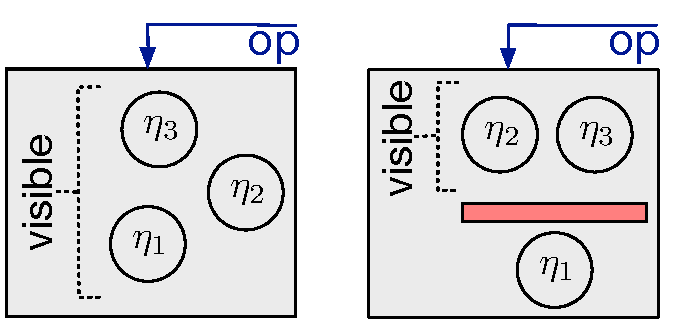
\includegraphics[scale=0.36]{Figures/ub.pdf}
	\end{subfigure}
	\caption{Filteration and \UB{} contracts}
\vspace{-5mm}
\label{fig:ub}
\end{figure}



  
